%%%%%%%%%%%%%%%%%%%%%%%%%%%%%%%%%%%%%%%%
%---------- Segundo Capitulo ----------
\chapter{Fundamenta\c{c}\~ao Te\'orica}
\label{chap:desenv}
%%%%%%%%%%%%%%%%%%%%%%%%%%%%%%%%%%%%%%%%

Com o objetivo de simular o efeito coro, al�m do \textit{SpeechEasy} que integra \textit{hardware} e \textit{software} \cite{Microson2015} num dispositivo eletr\^onico, existem algumas ferramentas que trabalham somente com \textit{software} e que exercem essa fun\c{c}\~ao juntamente com algum dispositivo de reprodu\c{c}\~ao de a\'udio que contenha microfone. 

Para computadores de mesa e notebooks com sistema operacional Windows, existe o "\textit{Software} Mais Flu\^encia Win DAF/FAF \textit{Software}", desenvolvida em 2009 pelo Henrique Confessor, \'e \textit{freeware} podendo ser distribu\'ida e utilizada livremente. Disponibilizada gratuitamente para \textit{download} no site da "Abra Gagueira" \cite{Confessor2009}.

\begin{figure}[H]
	\centering
	%\captionsetup{width=0.97\textwidth}
	\caption[Interface do software Mais Flu\^encia Win DAF/FAF]{Interface do software Mais Flu\^encia Win DAF/FAF. \label{fig:figuramaisfluencia}}
	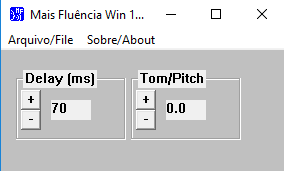
\includegraphics[height=7cm]{./Figuras/maisfluencia_figure.png}% <- formatos PNG, JPG e PDF
	\fonte{O Autor.}
\end{figure}

Para dispositivos m\'oveis com sistema operacional Android ou IOS existe o \textit{DAF Assistant} que tem uma vers\~ao gratuita, por\'em com limite de tempo para sua utiliza\c{c}\~ao, j\'a sua vers\~ao paga que n\~ao possui essa restri\c{c}\~ao, custa aproximadamente 13 reais na \textit{Play Store} e 33 reais no \textit{Itunes}, variando de acordo com pre�o do dollar \cite{Artefact2012}.

\begin{figure}[H]
	\centering
	%\captionsetup{width=0.97\textwidth}
	\caption[Interface do aplicativo DAF Assistant]{Interface do aplicativo DAF Assistant. \label{fig:figuradafassistant}}
	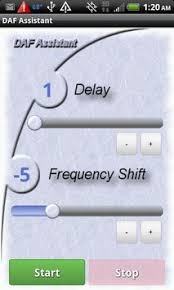
\includegraphics[height=10cm]{./Figuras/dafassistant_figure.jpg}% <- formatos PNG, JPG e PDF
	\fonte{\cite{Artefact2012}}
\end{figure}

Com o intuito de fornecer o \sigla{FAA}{\textit{feedback} auditivo atrasado}, existe o aplicativo "Terapia para a gagueira - FAA", que \'e gratuito e traz informa\c{c}\~oes interessantes sobre o tratamento da gagueira, como dicas de como utilizar o aplicativo e informa��es adicionais sobre tratamentos que melhoram a flu\^encia da fala. Lembrando que diferente da \sigla{RAA}{Retroalimenta\c{c}\~ao Auditiva Atrasada}, o FAA trabalha apenas com o atraso na reprodu��o da voz, n\~ao alterando a frequ\^encia com que a voz \'e reproduzida \cite{Age2017}. 

\begin{figure}[H]
	\centering
	%\captionsetup{width=0.97\textwidth}
	\caption[Interface do aplicativo Terapia para a gagueira - FAA]{Interface do aplicativo Terapia para a gagueira - FAA. \label{fig:figuraterapiaparagagueira}}
	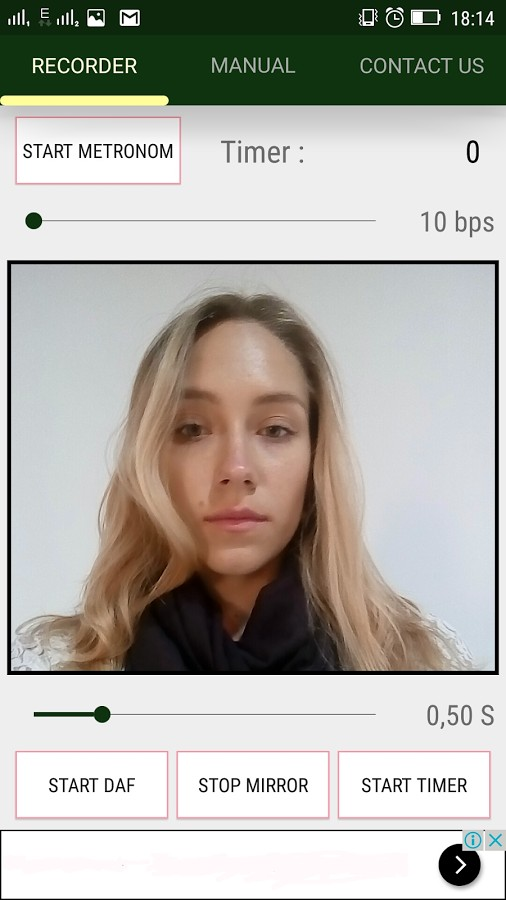
\includegraphics[height=10cm]{./Figuras/terapiaparagagueira_figure.jpg}% <- formatos PNG, JPG e PDF
	\fonte{\cite{Age2017}}
\end{figure}







